%% FullCourse_10Lecs -- Lecture 8, Topic 8.3: Vector Storage + Beyond Dense (GraphRAG)
%% Source: ./archive_pre_split/Lec08_RAG.tex (sections 7-8)
%% Pass B (2026-05-17): layered in refinements from
%%         ../../MiniCourse_8hr/Slides/Module4_Agentic_AI/M4_T2_Advanced_RAG_GraphRAG.tex
%% Ported frames:
%%   - "Knowledge Graph Triples: Examples Across Research Corpora" (corpus-specific triple table)
%%   - "Vanilla RAG vs. GraphRAG: A Direct Comparison" (question-type comparison table)
%%   - "Future Directions: Graph, Multimodal, Agentic" (closing 3-pillar frame)
%% All existing FullCourse frames are preserved.

%% Shared preamble for the FullCourse_10Lecs topic decks.
%%
%% Each topic .tex \input's this file, then defines its own \title, \date
%% override (if any), \graphicspath, and \begin{document}.
%%
%% Reconstructed verbatim from the inlined copy preserved in
%% Lec10_Case_Studies/Lec10_T8_Case6_DeepRamsey.tex (lines 23-190), which is
%% explicitly annotated there as "from ../shared_preamble.tex, copied verbatim".
%% Base preamble matches MiniCourse_8hr/Slides/shared_preamble.tex; this version
%% additionally provides \sectiondivider, the conceptbox/cautionbox/examplebox/
%% takeawaybox tcolorboxes, and \compacttables used across the split decks.

\documentclass[10pt,english,aspectratio=169]{beamer}

\usepackage{ae,aecompl}
\usepackage[T1]{fontenc}
\usepackage{textcomp}
\usepackage[utf8]{inputenc}
\usepackage{babel}
\usepackage{datetime2}

\setcounter{secnumdepth}{3}
\setcounter{tocdepth}{3}

\usepackage{amsmath, amssymb, amsthm, graphicx}
\usepackage{booktabs, multirow}
\usepackage{tikz}
\usepackage{pgfplots}
\pgfplotsset{compat=1.16}
\usepackage[most]{tcolorbox}
\tcbuselibrary{skins, breakable, theorems}
\usepackage{listings}
\usepackage{xcolor}

\lstset{
  basicstyle=\ttfamily\small,
  keywordstyle=\color{blue!80!black}\bfseries,
  commentstyle=\color{green!50!black}\itshape,
  stringstyle=\color{orange!80!black},
  backgroundcolor=\color{gray!8},
  frame=single,
  rulecolor=\color{gray!40},
  breaklines=true,
  showstringspaces=false,
  numbers=none,
}

\lstdefinestyle{pythonstyle}{
    language=Python,
    basicstyle=\ttfamily\footnotesize,
    keywordstyle=\color{blue!80!black}\bfseries,
    commentstyle=\color{green!50!black}\itshape,
    stringstyle=\color{orange!80!black},
    frame=single,
    breaklines=true,
    showstringspaces=false,
    numbers=left,
    numbersep=5pt,
    numberstyle=\tiny\color{gray},
    backgroundcolor=\color{gray!8},
    rulecolor=\color{gray!40}
}

\ifx\hypersetup\undefined
  \AtBeginDocument{%
    \hypersetup{bookmarks=false,breaklinks=true,pdfborder={0 0 0},colorlinks=true,
      linkcolor=DarkText,urlcolor=RedTitle}%
  }
\else
  \hypersetup{bookmarks=false,breaklinks=true,pdfborder={0 0 0},colorlinks=true,
    linkcolor=DarkText,urlcolor=RedTitle}%
\fi

\makeatletter
\newcommand\makebeamertitle{%
  \begin{frame}[plain]
    \vspace*{1.0cm}
    \centering
    {\usebeamerfont{title}\usebeamercolor[fg]{title}\inserttitle\par}
    \vspace{1.0cm}
    {\usebeamerfont{author}\usebeamercolor[fg]{author}\insertauthor\par}
    \vspace{0.2cm}
    {\usebeamerfont{date}\usebeamercolor[fg]{date}\insertdate\par}
  \end{frame}}%
\AtBeginDocument{%
  \let\origtableofcontents=\tableofcontents
  \def\tableofcontents{\@ifnextchar[{\origtableofcontents}{\gobbletableofcontents}}
  \def\gobbletableofcontents#1{\origtableofcontents}%
}

\usetheme{metropolis}
\usefonttheme{professionalfonts}

\definecolor{LightGray}{RGB}{230,230,230}
\definecolor{RedTitle}{RGB}{0,0,200}
\definecolor{VeryLightGray}{RGB}{245,245,245}
\definecolor{DarkText}{RGB}{0,0,0}

\setbeamercolor{background canvas}{bg=white}
\setbeamercolor{title}{fg=RedTitle}
\setbeamercolor{author}{fg=DarkText}
\setbeamercolor{date}{fg=DarkText}
\setbeamercolor{frametitle}{bg=VeryLightGray,fg=DarkText}
\setbeamercolor{normal text}{fg=DarkText}
\setbeamerfont{title}{size=\large}

\setbeamersize{text margin left=5mm, text margin right=5mm}
\addtobeamertemplate{frametitle}{}{\vspace{-0.5em}}
\newcommand{\reducevspace}{\vspace{-0.5cm}}

% Shared section divider and box styles for split topic decks.
\newcommand{\sectiondivider}[2]{%
\begin{frame}[plain,noframenumbering]
\begin{center}
\vfill
{\Large\textbf{#1}\par}
\vspace{0.35cm}
{\normalsize #2\par}
\vfill
\end{center}
\end{frame}
}

\newtcolorbox{conceptbox}[1][]{
  colback=blue!3,
  colframe=RedTitle!55,
  boxrule=0.35mm,
  arc=1mm,
  left=2mm,
  right=2mm,
  top=1mm,
  bottom=1mm,
  #1
}
\newtcolorbox{cautionbox}[1][]{
  colback=red!3,
  colframe=red!50!black,
  boxrule=0.35mm,
  arc=1mm,
  left=2mm,
  right=2mm,
  top=1mm,
  bottom=1mm,
  #1
}
\newtcolorbox{examplebox}[1][]{
  colback=green!3,
  colframe=green!45!black,
  boxrule=0.35mm,
  arc=1mm,
  left=2mm,
  right=2mm,
  top=1mm,
  bottom=1mm,
  #1
}
\newtcolorbox{takeawaybox}[1][]{
  colback=VeryLightGray,
  colframe=RedTitle!55,
  boxrule=0.35mm,
  arc=1mm,
  left=2mm,
  right=2mm,
  top=1mm,
  bottom=1mm,
  #1
}
\newcommand{\compacttables}{\renewcommand{\arraystretch}{1.15}}

\setbeamertemplate{navigation symbols}{}
\setbeamertemplate{footline}{%
  \hfill%
  \usebeamercolor[fg]{page number in head/foot}%
  \usebeamerfont{page number in head/foot}%
  \insertframenumber\,/\,\inserttotalframenumber\kern1em\vskip2pt%
}

\makeatother

\author{Zhigang Feng}
% "date with time": compile timestamp so each build is identifiable.
\date{\today\ \DTMcurrenttime}


\usetikzlibrary{arrows.meta, positioning, shapes.geometric, fit, calc, backgrounds}

% Macros for the ported GRAM (slides_v2.tex) four-mechanism diagram. \providecommand
% so nothing clashes with shared_preamble.tex.
\providecommand{\OLG}{OLG}
\providecommand{\LLM}{\textsc{llm}}
\providecommand{\RAG}{\textsc{rag}}
\providecommand{\GraphRAG}{\textsc{GraphRAG}}

\graphicspath{{./pic/}{./figures/}{../../MiniCourse_8hr/Slides/Module4_Agentic_AI/pic/}{../}}

\title[AI for Econ Research]{AI for Economic Research: Dynamic Models, Language, and Agents\\
Lecture 8.3: Vector Storage, Retrieval, and GraphRAG}

\begin{document}

\makebeamertitle

%=============================================================================
\begin{frame}{Topic 8.3 Agenda}
\begin{enumerate}
  \item \textbf{Vector Storage and Retrieval} --- vector DBs, ANN search
  \medskip
  \item \textbf{Beyond Dense Retrieval} --- hybrid, GraphRAG
\end{enumerate}

\medskip
\textit{Arc: T1 Prompting wall $\to$ T2 Chunking \& embeddings $\to$ \textbf{T3 Vector \& graph retrieval} $\to$ T4a Augmented generation $\to$ T4b Demo, failures, agentic bridge}
\end{frame}

%=============================================================================
\section{Vector Storage and Retrieval}

\begin{frame}{Why a Vector Database?}
\begin{itemize}
\item Now we have millions of chunks, each with a 1024-dim embedding. \textbf{Where do they live?}

\medskip
\item \textbf{The naive option:} a flat numpy array on disk. Search by computing cosine similarity to every vector and sorting.
\begin{itemize}
    \item Works fine for $10{,}000$ vectors.
    \item At $1{,}000{,}000$ vectors a single query takes seconds.
    \item At $10{,}000{,}000$ it is impractical.
    \item No metadata filters. No incremental updates. No persistence.
\end{itemize}

\medskip
\item \textbf{A vector database} solves all four:
\begin{enumerate}
    \item \emph{Scale:} approximate nearest-neighbor (ANN) algorithms search millions of vectors in milliseconds.
    \item \emph{Metadata filters:} restrict search to ``date $\geq$ 2020 AND doc\_type = minutes.''
    \item \emph{Incremental updates:} add new chunks as new documents arrive, without rebuilding the index.
    \item \emph{Persistence:} the index lives on disk and survives process restarts.
\end{enumerate}
\end{itemize}
\end{frame}

\begin{frame}{Vector DB Landscape --- Scale vs Hosting Cost}
\begin{center}
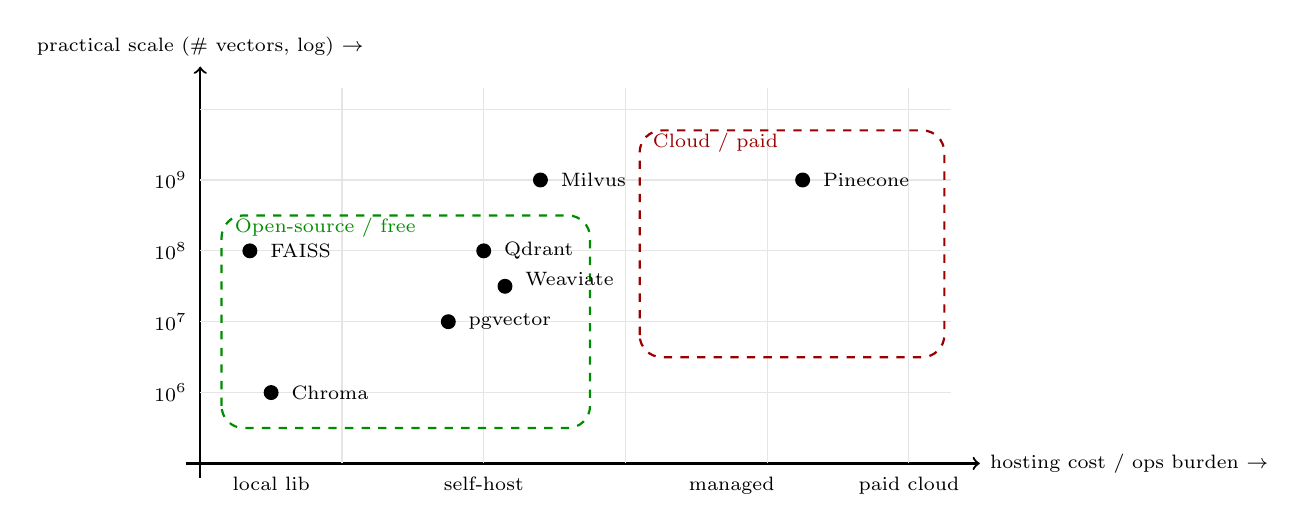
\begin{tikzpicture}[font=\footnotesize, scale=0.9]
  % axes
  \draw[->, thick] (-0.2,0) -- (11.0,0) node[right, font=\scriptsize] {hosting cost / ops burden $\to$};
  \draw[->, thick] (0,-0.2) -- (0,5.6) node[above, font=\scriptsize] {practical scale (\# vectors, log) $\to$};
  % grid
  \foreach \y in {1,2,3,4,5} \draw[gray!20] (0,\y) -- (10.6,\y);
  \foreach \x in {2,4,6,8,10} \draw[gray!20] (\x,0) -- (\x,5.3);

  % y-axis labels
  \node[font=\scriptsize, anchor=east] at (-0.05,1) {$10^6$};
  \node[font=\scriptsize, anchor=east] at (-0.05,2) {$10^7$};
  \node[font=\scriptsize, anchor=east] at (-0.05,3) {$10^8$};
  \node[font=\scriptsize, anchor=east] at (-0.05,4) {$10^9$};
  % x-axis labels
  \node[font=\scriptsize, anchor=north] at (1.0,-0.05) {local lib};
  \node[font=\scriptsize, anchor=north] at (4.0,-0.05) {self-host};
  \node[font=\scriptsize, anchor=north] at (7.5,-0.05) {managed};
  \node[font=\scriptsize, anchor=north] at (10.0,-0.05) {paid cloud};

  % Open-source ellipse (left + bottom-middle)
  \draw[draw=green!55!black, thick, dashed, rounded corners=8pt]
       (0.3,0.5) rectangle (5.5,3.5);
  \node[green!55!black, font=\scriptsize, anchor=south west] at (0.35,3.05) {Open-source / free};

  % Cloud / paid ellipse
  \draw[draw=red!60!black, thick, dashed, rounded corners=8pt]
       (6.2,1.5) rectangle (10.5,4.7);
  \node[red!60!black, font=\scriptsize, anchor=south west] at (6.25,4.25) {Cloud / paid};

  % Systems as dots
  \fill[black] (0.7,3.0) circle (3pt); \node[font=\scriptsize, anchor=west] at (0.85,3.0) {FAISS};
  \fill[black] (1.0,1.0) circle (3pt); \node[font=\scriptsize, anchor=west] at (1.15,1.0) {Chroma};
  \fill[black] (4.0,3.0) circle (3pt); \node[font=\scriptsize, anchor=west] at (4.15,3.0) {Qdrant};
  \fill[black] (4.3,2.5) circle (3pt); \node[font=\scriptsize, anchor=west] at (4.45,2.6) {Weaviate};
  \fill[black] (4.8,4.0) circle (3pt); \node[font=\scriptsize, anchor=west] at (4.95,4.0) {Milvus};
  \fill[black] (3.5,2.0) circle (3pt); \node[font=\scriptsize, anchor=west] at (3.65,2.0) {pgvector};
  \fill[black] (8.5,4.0) circle (3pt); \node[font=\scriptsize, anchor=west] at (8.65,4.0) {Pinecone};
\end{tikzpicture}
\end{center}

\medskip
\textbf{For an economist starting out:}
\begin{itemize}\small
\item \textbf{Chroma} or \textbf{FAISS} for laptop / cluster work --- bottom-left of the chart. Free, local, simple.
\item \textbf{pgvector} if you already manage a Postgres database --- middle of the open-source box. Reuses existing infra.
\item \textbf{Pinecone / Qdrant cloud} if you need a hosted index and have budget --- the right-hand cluster.
\end{itemize}
\end{frame}

\begin{frame}{Similarity Search 101}
\begin{itemize}
\item Given a query vector $q$ and a database of vectors $\{d_1, d_2, \dots, d_N\}$, find the $K$ closest $d_i$ to $q$.

\medskip
\item \textbf{Three common similarity functions:}
\begin{itemize}
    \item \textbf{Cosine similarity:} $\;\cos(\theta) = \dfrac{q \cdot d_i}{\|q\| \, \|d_i\|}$
    \item \textbf{Dot product:} $\;q \cdot d_i$
    \item \textbf{(Negative) Euclidean distance:} $\;-\|q - d_i\|$
\end{itemize}

\medskip
\item \textbf{Why cosine is the default:} Cosine is invariant to vector magnitude. Modern embedders are typically L2-normalized at the end of the forward pass, in which case cosine $=$ dot product and both reduce to: \emph{higher dot product $\Rightarrow$ more similar}.

\medskip
\item \textbf{Geometric picture:} Each chunk is an arrow from the origin. The query is another arrow. Cosine similarity measures the angle between them. Two vectors pointing in the same direction (small angle) are deemed similar regardless of length.
\end{itemize}
\end{frame}

\begin{frame}{Approximate Nearest Neighbor (ANN)}
\begin{itemize}
\item \textbf{Exact search} computes similarity to \emph{every} vector in the database. Cost: $O(N \cdot d)$ per query.

\medskip
\item For $N = 10^7$ and $d = 1024$, that's $\sim$$10^{10}$ floating-point operations per query --- seconds of latency.

\medskip
\item \textbf{Approximate Nearest Neighbor:} Sacrifice a tiny bit of accuracy ($\sim$1\% recall loss) for orders-of-magnitude speedup.

\medskip
\item \textbf{Two dominant ANN families:}
\begin{itemize}
    \item \textbf{HNSW} (Hierarchical Navigable Small World): build a multi-layer graph of vectors; search by greedy walks on the graph. Default in Qdrant, Weaviate, pgvector.
    \item \textbf{IVF} (Inverted File): cluster vectors into Voronoi cells, search only the closest cells. Default in FAISS for very large indexes.
\end{itemize}

\medskip
\item \textbf{In practice} you won't choose the algorithm by hand --- you'll pick a vector DB and accept its default. But knowing the names helps when you read the docs.
\end{itemize}
\end{frame}

\begin{frame}{Hybrid Retrieval: Dense + Sparse}
\begin{itemize}
\item \textbf{The dense-only failure case:} A user asks ``find every speech mentioning \emph{Section 13(3)}.'' This is a precise legal-citation query.
\begin{itemize}
    \item Dense embeddings cluster similar \emph{meanings}, not similar \emph{strings}.
    \item ``Section 13(3)'' may not even be in the embedder's vocabulary.
    \item Result: top-10 neighbors are about the discount window in general --- not the specific section.
\end{itemize}

\medskip
\item \textbf{The fix:} also run a classical sparse retriever in parallel.
\begin{itemize}
    \item \textbf{BM25}: a TF-IDF-based ranking function that scores documents by exact term matches with the query.
    \item Catches everything dense retrieval misses on rare strings, acronyms, statute citations, ticker symbols, identifiers.
\end{itemize}

\medskip
\item \textbf{Combine the two via Reciprocal Rank Fusion (RRF):}
\[
\text{score}(d) = \sum_{r \in \{\text{dense, sparse}\}} \frac{1}{k + \text{rank}_r(d)}
\quad \text{(typically } k = 60 \text{)}
\]

\medskip
\item Hybrid retrieval is the \textbf{production default in 2025}. Pure dense is rarely competitive.
\end{itemize}
\end{frame}

\begin{frame}{Re-Ranking with Cross-Encoders}
\begin{itemize}
\item \textbf{Two-stage retrieval:}
\begin{enumerate}
    \item \textbf{First pass (bi-encoder):} fast, embeds query and documents \emph{independently}, returns top-50 candidates by cosine similarity.
    \item \textbf{Second pass (cross-encoder re-ranker):} slow, takes the query \emph{and} a candidate document \emph{together} as input, outputs a relevance score. Returns the top-5.
\end{enumerate}

\medskip
\item \textbf{Why this works.} A cross-encoder reads the query and document jointly --- so it can attend to which parts of the document actually answer the query. Bi-encoders cannot do this. The cost: cross-encoders are $\sim$100$\times$ slower per pair, so we only use them on the top-50 short-list.

\medskip
\item \textbf{Popular re-rankers:}
\begin{itemize}
    \item Cohere \texttt{Rerank} (paid API)
    \item \texttt{bge-reranker-large} (free, local)
    \item \texttt{ms-marco-MiniLM-L-12-v2} (free, smaller)
\end{itemize}

\medskip
\item \textbf{Why re-ranking matters in practice.} The top-1 hit from a bi-encoder is often outranked by something the re-ranker catches. Without re-ranking you ask the LLM the wrong question.
\end{itemize}
\end{frame}

\begin{frame}{Metadata Filters}
\begin{itemize}
\item Pure semantic search is insufficient when the query has \emph{structural} constraints.

\medskip
\item \textbf{Real example:} \emph{``Find all FOMC discussions of unemployment from 2020 onwards, excluding press conferences.''}
\begin{itemize}
    \item ``Discussions of unemployment'' $\Rightarrow$ semantic search.
    \item ``From 2020 onwards'' $\Rightarrow$ filter on \texttt{date $\geq$ 2020-01-01}.
    \item ``Excluding press conferences'' $\Rightarrow$ filter on \texttt{doc\_type $\neq$ press\_conference}.
\end{itemize}

\medskip
\item Modern vector DBs let you combine vector similarity with SQL-style metadata filters in a single query.

\medskip
\item \textbf{This is exactly why preserving rich metadata at chunking time matters} (Section IV gotcha). If your chunks don't carry \texttt{date}, \texttt{doc\_type}, \texttt{speaker}, etc., you cannot filter on them later.

\medskip
\item \textbf{Rule of thumb:} Add \emph{more} metadata than you think you need. It is cheap at index time and impossible to reconstruct after the fact.
\end{itemize}
\end{frame}

\begin{frame}[fragile]{Code: Build a Chroma Index and Query It}
\begin{lstlisting}[language=Python]
import chromadb
from sentence_transformers import SentenceTransformer

model = SentenceTransformer("BAAI/bge-large-en-v1.5")

# 1. Persistent Chroma client (data lives on disk)
client = chromadb.PersistentClient(path="./fomc_index")
coll = client.get_or_create_collection("fomc")

# 2. Add chunks with metadata
coll.add(
    ids=[f"chunk_{i}" for i in range(len(chunks))],
    documents=chunks,
    embeddings=model.encode(chunks, normalize_embeddings=True).tolist(),
    metadatas=[{"meeting": "2024-06", "doc_type": "minutes"} for _ in chunks],
)

# 3. Query: "How did the Committee discuss inflation expectations?"
query = "How did the Committee discuss inflation expectations?"
q_emb = model.encode([query], normalize_embeddings=True).tolist()

results = coll.query(
    query_embeddings=q_emb,
    n_results=5,
    where={"doc_type": "minutes"},   # metadata filter
)

for doc, meta in zip(results["documents"][0], results["metadatas"][0]):
    print(meta["meeting"], "->", doc[:80])
\end{lstlisting}
\end{frame}

%=============================================================================
\section{Beyond Dense Retrieval}

\begin{frame}{Where Vanilla Vector RAG Starts to Break}
\begin{itemize}
\item Dense retrieval is a \textbf{local similarity machine}. It finds chunks whose wording or meaning is close to the query.

\medskip
\item That is enough for many lookup questions, but it misses three important structures:
\begin{enumerate}
    \item \textbf{Relationships between objects.} Two chunks may matter because their entities are linked, even if the wording differs.
    \item \textbf{Global structure.} Nearest-neighbor search has no notion of discourse communities, themes, or argument clusters across an entire corpus.
    \item \textbf{Coverage.} If the same fact appears in many chunks, top-$K$ retrieval often returns duplicates instead of a representative overview.
\end{enumerate}

\medskip
\item \textbf{Economist examples:}
\begin{itemize}
    \item ``Which Senators most often connect inflation to housing supply constraints?''
    \item ``What are the main camps in recent papers on LLMs and education?''
\end{itemize}

\medskip
\item Once the question is \textbf{multi-hop} or \textbf{corpus-level}, plain top-$K$ chunk retrieval is often the wrong abstraction.
\end{itemize}
\end{frame}

\begin{frame}{Concrete Break Point: Where Vanilla Fails (and Why GraphRAG Follows)}
\textbf{Question:} \emph{``Which Phillips-curve papers use survey expectations and are cited by post-2020 FOMC speeches?''}

\medskip
\begin{columns}[T,totalwidth=\textwidth]
\column{0.49\textwidth}
\textbf{Vanilla vector RAG}
\begin{itemize}\small
\item Embeds the query as one vector.
\item Returns 5 chunks that \emph{sound like} ``Phillips curve + survey expectations.''
\item Has \textbf{no notion of citation edges} between NBER papers and FOMC speeches.
\item Best-case output: a chunk that \emph{discusses} both topics, even if no actual citation link exists.
\item Failure mode: confident, fluent, but the cited link is fictional.
\end{itemize}

\column{0.49\textwidth}
\textbf{GraphRAG}
\begin{itemize}\small
\item Walks the citation graph: NBER paper $\to$ \texttt{cited\_by} edge $\to$ FOMC speech node.
\item Filters by node attribute: \texttt{date $\geq$ 2020}.
\item Filters by paper attribute: \texttt{uses\_data: SurveyOfProfessionalForecasters} or similar.
\item Returns the actual subgraph; only then runs generation on the supporting chunks.
\item Failure mode: degrades to ``no path found,'' not invention.
\end{itemize}
\end{columns}

\vspace{0.25cm}
\begin{takeawaybox}
\textbf{Rule:} reach for GraphRAG when the question is \emph{about a relationship}, not just \emph{about a topic}. Top-$K$ similarity cannot manufacture an edge that the index does not represent.
\end{takeawaybox}
\end{frame}

\begin{frame}{Knowledge Graphs: Adding Structure to Retrieval}
\begin{columns}[T,totalwidth=\textwidth]
\column{0.50\textwidth}
\begin{itemize}
\item A \textbf{knowledge graph (KG)} stores facts as \textbf{nodes + edges} rather than isolated chunks.

\medskip
\item Canonical representation: \texttt{<head, relation, tail>}, e.g.\
\texttt{<Powell, discusses, inflation expectations>}.

\medskip
\item In graph-based RAG, the index can mix \textbf{entity nodes}, \textbf{chunk nodes}, and \textbf{community summaries}.

\medskip
\item The gain is simple: retrieval is no longer ``find text that sounds similar.'' It becomes ``find the \emph{relevant subgraph}.''
\end{itemize}

\column{0.46\textwidth}
\centering

\includegraphics[width=\linewidth]{graph_rag_share/knowledge_graph_example.png}

\scriptsize
Once facts are stored as a graph, retrieval can follow links rather than isolated paragraphs.
\end{columns}
\end{frame}

\begin{frame}{Graph-Based RAG: Offline vs.\ Online}
\begin{columns}[T,totalwidth=\textwidth]
\column{0.34\textwidth}
\small
\textbf{Offline indexing}
\begin{itemize}
    \item chunk the corpus
    \item extract entities and relations
    \item build the graph and any auxiliary indexes
    \item optionally detect communities and summarize them
\end{itemize}

\textbf{Online querying}
\begin{itemize}
    \item interpret or rewrite the question
    \item retrieve nodes, edges, chunks, or communities
    \item expand to a relevant subgraph
    \item build the prompt and ask the LLM to answer
\end{itemize}

\column{0.62\textwidth}
\centering

\includegraphics[width=\linewidth]{graph_rag_share/graphrag_pipeline.png}

\scriptsize
GraphRAG-style intuition: communities are built offline, then query-focused summaries are composed online.
\end{columns}
\end{frame}

\begin{frame}{Knowledge Graph Triples: Examples Across Research Corpora}
\small
\textbf{Once relationships are explicit, retrieval can follow links, communities, paths, and neighborhoods --- not only semantic distance.}

\vspace{0.1cm}
\begin{center}
\footnotesize
\begin{tabular}{|p{3.8cm}|p{8.6cm}|}
\hline
\textbf{Corpus} & \textbf{Example triples} \\ \hline
FOMC archive & \texttt{<June 2024 minutes, discusses, inflation expectations>} \\
             & \texttt{<Powell press conference, mentions, labor-market rebalancing>} \\ \hline
NBER / RePEc papers & \texttt{<Paper A, estimates, Phillips curve slope>} \\
                    & \texttt{<Paper A, uses data, CPS>} \\
                    & \texttt{<Paper B, cites, Paper A>} \\ \hline
SEC filings & \texttt{<Bank X 10-K, reports risk, deposit beta>} \\
            & \texttt{<Bank X, exposed to, commercial real estate>} \\ \hline
Central bank speeches & \texttt{<ECB speech 2022-09, frames, transitory inflation>} \\
                      & \texttt{<Lagarde, cited by, FOMC speakers>} \\ \hline
\end{tabular}
\end{center}

\vspace{0.05cm}
\textbf{Why it matters for economists:} Questions like \emph{``Which Phillips-curve papers use survey expectations and are cited by post-2020 FOMC speeches?''} are \emph{graph queries}, not semantic-similarity queries.
\end{frame}

\begin{frame}{Vanilla RAG vs.\ GraphRAG: A Direct Comparison}
\small
\begin{center}
\footnotesize
\begin{tabular}{|p{3.2cm}|p{4.6cm}|p{5.2cm}|}
\hline
\textbf{Question type} & \textbf{Vector / hybrid RAG} & \textbf{GraphRAG} \\ \hline
Specific fact lookup & Strong when the exact chunk is nearby & Strong if fact is attached to an entity or path \\ \hline
Relationship query & Often requires several retrieved chunks and luck & Natural: traverse edges and retrieve neighborhoods \\ \hline
Global summarization & Top-$K$ chunks under-cover the corpus & Community reports summarize modules of the corpus \\ \hline
High redundancy corpus & May retrieve near-duplicate boilerplate & Can collapse repeated facts into entities/communities \\ \hline
Cost and complexity & Simpler, cheaper, easier to debug & More expensive offline; KG quality matters \\ \hline
\end{tabular}
\end{center}

\vspace{0.15cm}
\textbf{Research rule:} start with vector + BM25 + re-rank. Move to graph or hierarchical retrieval \emph{only} when the question requires relationships or corpus-level themes you can't get from local similarity.
\end{frame}

%=============================================================================
% Research case study: GRAM (GraphRAG over the OLG economics literature).
% Ported/adapted from the instructor's research deck
% (llm_econ_modelling/draft/slides/slides_v2.tex). Framed as the research-grade
% escalation of the toy OLG demo in T4b. Headline metrics are forthcoming, so
% the condition-aware advantage is presented as a DESIGN GOAL, not a measured win.
%=============================================================================

\begin{frame}{Case Study: GraphRAG over the OLG Economics Literature (GRAM)}
\begin{itemize}
\item A research-grade GraphRAG --- the instructor's own \textbf{GRAM} project --- built over a curated \textbf{157-paper overlapping-generations (OLG)} macro corpus. Think of it as the \emph{research-grade escalation} of the small offline OLG demo coming in Topic 8.4b, not a replacement.

\medskip
\item \textbf{One running query} (we trace it through four mechanisms next):
\begin{quote}\itshape\small
``An OLG life-cycle model with idiosyncratic \emph{and} aggregate shocks and incomplete intergenerational asset markets --- which solver class is admissible for the joint stationary distribution in recursive equilibrium?''
\end{quote}

\item \textbf{Why economics is special:} every paper is \textbf{math} (the analytical scaffold) \emph{and} \textbf{prose} (the mechanism). \emph{Math is analysis; prose is mechanism.}
\begin{itemize}\small
    \item Math-IR systems retrieve theorems/equations; legal/clinical RAG retrieves prose. An econ assistant needs \emph{both}.
    \item GRAM sits between those worlds: a domain-typed graph over economic models.
\end{itemize}
\end{itemize}
\end{frame}

\begin{frame}{Four Context Mechanisms on One Query}
\footnotesize\itshape
``\OLG{} life-cycle, idiosyncratic $+$ aggregate shocks, incomplete intergenerational asset markets --- which solver class is admissible for the joint stationary distribution in recursive equilibrium?''
\normalfont
\begin{center}
\resizebox{!}{0.60\textheight}{%
\begin{tikzpicture}[
  font=\footnotesize,
  node distance=2.4mm,
  q/.style       ={draw,rounded corners=1pt,inner sep=2pt,minimum width=20mm,minimum height=4.5mm,fill=gray!5},
  corpus/.style  ={draw,rounded corners=0.5pt,inner sep=2pt,minimum width=20mm,minimum height=4.5mm,fill=red!10,align=center},
  pasted/.style  ={draw,rounded corners=0.5pt,inner sep=2pt,minimum width=20mm,minimum height=4.5mm,fill=yellow!22,align=center},
  vdb/.style     ={cylinder,shape border rotate=90,draw,aspect=0.22,minimum width=20mm,minimum height=11mm,fill=gray!18,font=\footnotesize,align=center,inner sep=1pt},
  kgicon/.style  ={draw,rounded corners=1pt,inner sep=2pt,minimum width=20mm,minimum height=11mm,fill=green!14,align=center},
  ctx/.style     ={draw,rounded corners=1pt,inner sep=1.5pt,minimum width=20mm,minimum height=4.5mm,fill=yellow!25,font=\scriptsize\itshape,align=center},
  llm/.style     ={draw,rounded corners=1pt,inner sep=2pt,minimum width=20mm,minimum height=4.5mm,fill=blue!14,align=center},
  ans/.style     ={draw,rounded corners=1pt,inner sep=2pt,minimum width=20mm,minimum height=4.5mm,fill=gray!5,align=center},
  outcome/.style ={text width=24mm,align=center,font=\scriptsize\itshape,text=gray!50!black},
  arr/.style     ={-{Latex[length=1.5mm]},semithick},
  hdr/.style     ={font=\footnotesize\bfseries,align=center,text width=24mm},
  gnode/.style   ={circle,inner sep=0pt,minimum size=1.2mm,fill=green!60!black}
]
\node[hdr] (h1) at (0,0) {Naive\\\LLM};
\node[q,below=of h1] (q1) {query};
\node[llm,below=of q1] (l1) {\LLM};
\node[ans,below=of l1] (a1) {answer};
\node[outcome,below=1mm of a1] {silent\\structural failure};
\draw[arr] (q1) -- (l1); \draw[arr] (l1) -- (a1);

\node[hdr] (h2) at (2.85,0) {In-context\\stuffing};
\node[pasted,below=of h2] (cp2) {pasted\\excerpts};
\node[ctx,below=4mm of cp2] (ctx2) {query + pasted text};
\node[llm,below=of ctx2] (l2) {\LLM};
\node[ans,below=of l2] (a2) {answer};
\node[outcome,below=1mm of a2] {bounded by\\user curation};
\draw[arr] (cp2) -- (ctx2); \draw[arr] (ctx2) -- (l2); \draw[arr] (l2) -- (a2);

\node[hdr] (h3) at (5.7,0) {\RAG\\(embedding)};
\node[corpus,below=of h3] (cp3) {literature};
\node[vdb,below=4mm of cp3] (vdb3) {embeddings};
\node[ctx,below=4mm of vdb3] (ctx3) {query + top-$k$\\passages};
\node[llm,below=of ctx3] (l3) {\LLM};
\node[ans,below=of l3] (a3) {answer};
\node[outcome,below=1mm of a3] {wrong-by-prominence};
\draw[arr] (cp3) -- (vdb3); \draw[arr] (vdb3) -- (ctx3); \draw[arr] (ctx3) -- (l3); \draw[arr] (l3) -- (a3);

\node[hdr] (h4) at (8.55,0) {\GraphRAG\\(GRAM)};
\node[corpus,below=of h4] (cp4) {literature};
\node[kgicon,below=of cp4] (kg4) {};
\node[font=\scriptsize] at ($(kg4.north)+(0,-1.6mm)$) {typed graph};
\node[gnode] (g1) at ($(kg4.center)+(-4mm,-2mm)$) {};
\node[gnode] (g2) at ($(kg4.center)+(0mm,-2.5mm)$) {};
\node[gnode] (g3) at ($(kg4.center)+(4mm,-2mm)$) {};
\node[gnode] (g4) at ($(kg4.center)+(-2mm,0.3mm)$) {};
\node[gnode] (g5) at ($(kg4.center)+(2mm,0.3mm)$) {};
\draw[gray!55,thin] (g1)--(g2) (g2)--(g3) (g4)--(g2) (g5)--(g2) (g1)--(g4) (g3)--(g5);
\node[ctx,below=of kg4] (ctx4) {query + ranked\\subgraph};
\node[llm,below=of ctx4] (l4) {\LLM};
\node[ans,below=of l4] (a4) {cited\\answer};
\node[outcome,below=1mm of a4,text=green!45!black] {ranked $+$\\condition-aware};
\draw[arr] (cp4) -- (kg4); \draw[arr] (kg4) -- (ctx4); \draw[arr] (ctx4) -- (l4); \draw[arr] (l4) -- (a4);
\end{tikzpicture}}
\end{center}
\end{frame}

\begin{frame}{Wrong-by-Prominence vs.\ Condition-Aware Retrieval}
\begin{itemize}
\item \textbf{Wrong-by-prominence:} pure embedding retrieval routes the query to the \emph{modal} (most-prominent) paper, regardless of whether it fits the asked-for conditions:
\begin{itemize}\small
    \item ``OLG with capital'' $\Rightarrow$ Diamond (1965), \emph{not} Auerbach--Kotlikoff (1987).
    \item ``heterogeneous-agent macro'' $\Rightarrow$ Aiyagari, \emph{not} Krusell--Smith.
\end{itemize}
\emph{The vocabulary is present; the applicability filter is absent.}

\medskip
\item \textbf{Condition-aware:} admissibility is \emph{conditional} --- change one model assumption (e.g.\ add aggregate risk) and a different solver class becomes admissible. Embedding similarity cannot encode that dependency; a walk over a \emph{typed} graph of model objects can.
\end{itemize}

\begin{takeawaybox}
\textbf{Honest framing.} ``Wrong-by-prominence'' and ``condition-aware'' name each mechanism's \emph{failure mode} on this query type. GRAM's condition-aware advantage over vanilla RAG is the \textbf{gap a planned three-condition evaluation (naive / RAG / GraphRAG) is designed to measure} --- a design goal and hypothesis, not yet a reported win.
\end{takeawaybox}
\end{frame}

\begin{frame}{Elements, Not Chunks: A Typed Retrieval Unit}
\begin{itemize}
\item Standard RAG (Topic 8.2) embeds a \textbf{$\sim$512-token text chunk}. GRAM's retrieval unit is a typed \textbf{element}.

\medskip
\item \textbf{The PromptEcon schema:} 3 phases (Environment $\to$ Equilibrium \& solution $\to$ Quantification), \textbf{9 categories}, \textbf{51 elements}, \textbf{7 typed edges} (\texttt{enters\_objective}, \texttt{enters\_constraint}, \texttt{clears\_in}, \texttt{derives}, \ldots).

\item Each paper $\to$ one provenance-carrying JSON of element records (\texttt{canonical\_name}, prose description with inline \TeX{}, \texttt{source\_lines}). \textbf{One embedding per element}, not per chunk; cross-paper merge happens at \texttt{(element, canonical\_name)}, not paper-level similarity.

\medskip
\item \textbf{Why it matters:} a chunk returns surface phrases (``aggregate shocks,'' ``recursive equilibrium'') without saying \emph{what enters which constraint} or \emph{what clears in which market}. Typed elements + edges preserve exactly that structure.
\end{itemize}
\begin{takeawaybox}
\textbf{Slogan:} \emph{the schema is the research; extraction is the mechanical pass.} The 9$\times$51 vocabulary is human-curated from five textbook traditions; per-paper instantiation is automated.
\end{takeawaybox}
\end{frame}

\begin{frame}{Corpus Construction as Engineering (Not Bibliography)}
\textbf{``A retrieval system is only as good as the documents in its index.''} GRAM treats corpus building as engineering with input contracts, artifacts, and acceptance tests.
\begin{itemize}
\item \textbf{157 papers}, three tiers (Foundations 12 / pre-2010 core 55 / published 2010+ 43 / frontier WPs 47); a 4-attribute model-class \emph{inclusion gate} fixes each paper's role.

\medskip
\item \textbf{Three design constraints worth copying:}
\begin{enumerate}\small
    \item \emph{Coverage vs.\ focus} --- index the full mechanism vocabulary, not the curator's reading list.
    \item \emph{Post-cutoff share} --- a non-trivial fraction (here 34 entries dated $>$2024) must post-date the LLM's training cutoff, so RAG can \emph{demonstrably} add value.
    \item \emph{Citation connectivity} --- documents must actually cite each other, or graph-traversal retrieval cannot reach them.
\end{enumerate}

\medskip
\item Reproducible by construction: every keep/drop decision logged; an 11-criterion acceptance audit (passed 9/11); MinerU for layout-aware PDF$\to$Markdown (math preserved); Qwen3-Embedding-8B ($\sim$\$0.25 to vectorize the pilot corpus).
\end{itemize}
\begin{takeawaybox}
\textbf{Caveats.} GRAM is \emph{one} research pipeline (the instructor's), shown beside Microsoft GraphRAG / LightRAG / HippoRAG / RAPTOR above --- not a canonical standard. It is unpublished, in-progress work; the figures here (157 papers, 9/11, tooling) are point-in-time facts for this pilot.
\end{takeawaybox}
\end{frame}

\begin{frame}{Choosing the Retrieval Architecture}
\begin{center}
\renewcommand{\arraystretch}{1.25}
\small
\begin{tabular}{|p{3.2cm}|p{3.1cm}|p{5.8cm}|}
\hline
\textbf{Question type} & \textbf{Best first choice} & \textbf{Why} \\
\hline
Precise factual lookup or citation hunt & Hybrid dense + sparse RAG & Exact strings, dates, and citations matter more than global structure. \\
\hline
Specific multi-hop entity question & Graph-based RAG & The answer depends on linked entities, paths, or neighborhoods rather than one chunk. \\
\hline
Broad abstract summarization over a large corpus & GraphRAG / RAPTOR-style hierarchy & You need coverage of themes or communities, not just the closest paragraphs. \\
\hline
Fast prototype on a changing corpus & Vanilla RAG first & A flat vector index is easy to build and update; add graph structure only if it buys real accuracy. \\
\hline
\end{tabular}
\end{center}

\bigskip
\textbf{Rule of thumb:} start with hybrid dense+sparse RAG. Escalate to graph or hierarchical retrieval when the task requires \emph{relationships}, \emph{coverage}, or \emph{multi-hop reasoning}.
\end{frame}

\begin{frame}{Representative Systems You Should Recognize}
\begin{center}
\renewcommand{\arraystretch}{1.2}
\scriptsize
\begin{tabular}{|p{2.0cm}|p{3.2cm}|p{2.7cm}|p{4.2cm}|}
\hline
\textbf{System} & \textbf{Core idea} & \textbf{Best at} & \textbf{What to remember} \\
\hline
Microsoft GraphRAG & Build a KG, detect communities, summarize them, then retrieve by community plus local evidence & Query-focused summarization & Strong when the user asks for an overview of a large corpus rather than one citation. \\
\hline
LightRAG & Dual-level retrieval: local entity-level evidence plus high-level thematic evidence & Mixed local/global questions & A pragmatic design that tries to keep graph retrieval lightweight. \\
\hline
HippoRAG & Expand a memory graph with KNN links, then run personalized PageRank from the query & Multi-hop recall & Explicitly treats retrieval as traversing associative memory. \\
\hline
RAPTOR & Recursively cluster chunks and summarize the clusters into a tree & Long-document and abstract QA & Not a full KG, but the same core idea: retrieve from higher-level structure when chunks alone are too local. \\
\hline
\end{tabular}
\end{center}

\medskip
\footnotesize
Key references: Edge et al.\ (2024), Guo et al.\ (2024), Gutierrez et al.\ (2024), and Sarthi et al.\ (2024).
\end{frame}

\begin{frame}{Visual Snapshots: GraphRAG and LightRAG}
\begin{columns}[T,totalwidth=\textwidth]
\column{0.49\textwidth}
\textbf{GraphRAG}


\includegraphics[width=0.96\linewidth]{graph_rag_share/graphrag_pipeline.png}

\scriptsize Community summaries provide global coverage for abstract questions.

\column{0.49\textwidth}
\textbf{LightRAG}


\includegraphics[width=\linewidth]{graph_rag_share/lightrag_workflow.png}

\scriptsize Dual-level retrieval: local entities plus higher-level themes.
\end{columns}
\end{frame}

\begin{frame}{Visual Snapshots: HippoRAG and RAPTOR}
\begin{columns}[T,totalwidth=\textwidth]
\column{0.49\textwidth}
\textbf{HippoRAG}


\includegraphics[width=\linewidth]{graph_rag_share/hipporag_workflow.png}

\scriptsize Personalized PageRank expands a memory-like graph neighborhood.

\column{0.49\textwidth}
\textbf{RAPTOR}


\includegraphics[width=\linewidth]{graph_rag_share/raptor_tree.png}

\scriptsize Recursive clustering and summarization into a tree.
\end{columns}
\end{frame}

\begin{frame}{What Recent Graph-RAG Benchmarks Suggest}
\begin{columns}[T,totalwidth=\textwidth]
\column{0.40\textwidth}
\small
\begin{itemize}
\item \textbf{Chunk quality still dominates.} Better chunks help almost every architecture.

\medskip
\item \textbf{High-level structure helps abstract questions.} Community reports and hierarchies beat a bag of similar chunks when the user wants synthesis.

\medskip
\item \textbf{Specific QA can still need structure.} Hard factual questions often require linking several local pieces of evidence.

\medskip
\item \textbf{Graph maintenance is expensive.} Build cost, token cost, and dynamic updates remain real bottlenecks.
\end{itemize}

\column{0.56\textwidth}
\centering

\includegraphics[width=\linewidth]{graph_rag_share/benchmark_efficiency.png}

\scriptsize
Illustrative benchmark from the donor deck: graph-RAG variants can buy capability, but often at sharply different token and latency costs.
\end{columns}
\end{frame}

\begin{frame}{Future Directions: Graph, Multimodal, Agentic}
\small
\begin{columns}[T]
\begin{column}{0.32\textwidth}
\textbf{Better graphs}
\begin{itemize}
    \item Higher-quality entity and relation extraction
    \item Attribute-rich nodes and edges
    \item Efficient incremental updates as new docs arrive
\end{itemize}
\end{column}
\begin{column}{0.32\textwidth}
\textbf{Richer evidence}
\begin{itemize}
    \item Tables, figures, equations, and PDFs
    \item Cross-modal alignment of text and data
    \item Provenance-preserving retrieval
\end{itemize}
\end{column}
\begin{column}{0.32\textwidth}
\textbf{Agentic RAG}
\begin{itemize}
    \item Agent chooses vector vs.\ graph vs.\ web
    \item Query rewriting and retrieval loops
    \item Automatic parameter tuning and evals
\end{itemize}
\end{column}
\end{columns}

\bigskip
\textbf{Macro research anchor:} A serious literature- or policy-text assistant will eventually need all three --- graph structure for relationships, multimodal parsing for papers and reports, and an agent loop for difficult questions.

\medskip
\textbf{Next (Topic 8.4a):} augmented generation --- how the retrieved evidence becomes a cited, refusable answer, and five economic-applications walkthroughs. \textbf{Topic 8.4b} then runs the OLG demo and bridges to \emph{Lecture 9}'s agentic loop.
\end{frame}

\end{document}
